\subsection{De behuizing}
\subsubsection{Voordeel voor de klant/ gebruiker van ...}
Al snel speelde het idee binnen de groep om een behuizing te maken waar de luidspreker en alle electronica in kon worden geplaatst. Het oorspronkelijke plan was om de behuizing te maken met behulp van een 3D-printer. Hierin zou de speaker geschroefd worden en de elektronica binnen de behuizing verwerkt worden. Op deze manier zouden we als resultaat een eindproduct krijgen wat zo compact mogelijk is en een duidelijk geheel is. 
Het voordeel van dit idee is dat de klant een makkelijk pakket krijgt waar alle elektronica achter de schermen is verwerkt. Hiernaast is de behuizing mooi en professioneel met een deksel die open gemaakt kan worden om de binnenkant te kunnen bekijken of bewerken. 

Het idee heeft echter ook een aantal belangrijke nadelen. Zulke grote behuizingen printen kost relatief veel geld. En het was voor het team niet mogelijk om een mooi design te creëren wat deze kosten aanvaardbaar maakt. Het zou een simpele doos worden van duur materiaal. Ander materiaal zou voor deze taak dus beter geschikt zijn. 
\begin{figure}[ht]
    \centering
    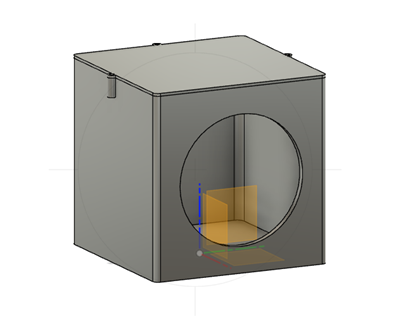
\includegraphics[width=0.90\textwidth]{IMG/004/v4.png}
    \caption{3D-model}
    \label{fig:3D-model}
\end{figure}

Na onderzoek te hebben gedaan zijn we op een betere en makkelijkere oplossing gekomen voor ons probleem. We kwamen te weten dat het gemakkelijk en goedkoop is om een soortgelijke doos te maken met houten platen die op een speciale manier worden verwerkt met een lasersnijder. Zo kan men heel accuraat het hout bewerken en er in dit geval een doos mee maken. Het voordeel hiervan is dat het zeer goedkoop is en een veel korter productieproces heeft. Dit zorgt ervoor dat de klant minder hoeft te betalen en er meer voorraad gemaakt kan worden in dezelfde tijd.

\subsubsection{Nadelen kosten van ...}
Er zijn in het huidige model nog wel nadelen ten opzichte van het 3D ontwerp. Zo hebben we op dit moment geen deksel die na assemblage er ook weer gemakkelijk af kan. Dit zal voor de gemiddelde klant geen probleem zijn maar zal het moeilijker maken om eventuele reparaties te verrichten. 

\subsubsection{Hoe werkt ... en hoe ziet ... er uit}
Het model gaat om 6 speciaal ontworpen plankjes die samengevoegd kunnen worden tot behuizing. De lasersnijder is zo accuraat dat er niet eens lijm nodig is om de doos stevig genoeg te laten worden, de wrijving en structuur maat het doosje al stevig. De elektronica zal aan de binnenkant worden verwerkt. Voor electronica die visueel beschikbaar moeten zijn zoals de LEDS en Display worden gaten geboord zodat deze van buiten de doos zichtbaar zullen worden. Op moment van schrijven zijn we in het assemblageproces wat op tijd klaar zal zijn voor de demonstratie op 24 januari. Hieronder is op verschillende foto’s te zien hoe de behuizing in elkaar zit. Ook wordt duidelijk hoe de luidspreker vast zit en waar de elektronica komt. Deze zijn op de foto echter nog niet vast gemaakt.

\begin{figure}[ht]
    \centering
    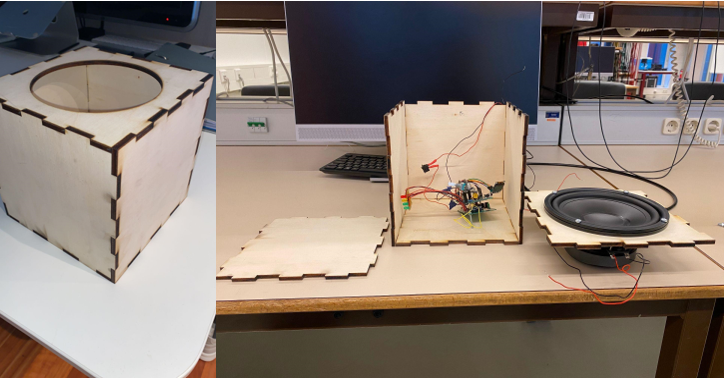
\includegraphics[width=0.90\textwidth]{IMG/004/v5.PNG}
    \caption{Behuizing}
    \label{fig:Behuizing}
\end{figure}